\begin{document}
\begin{abstract}

This paper presents a measurement of Johnson–Nyquist noise. Johnson–Nyquist noise, sometimes referred to as thermal noise, is defined as the electronic noise generated by the thermal agitation of the charge carriers inside an electrical conductor at equilibrium. As thermal noise is intrinsic to every electric circuit, it can act as a limiting factor on the sensitivity of electrical measuring instruments and could potentially drown out weak signals in sensitive electronic equipment. In a series of experiments, we measure the total noise recorded across various resistors. By fitting the cross-spectral density of the data to a quadratic model, we are able to extract Johnson noise and distinguish its contribution from the other sources of noise in the circuit. We then use Nyquist's theorem to derive a value for the Boltzmann constant $k_b$ that is in acceptable agreement with its literature value. 
\end{abstract}

% insert suggested PACS numbers in braces on next line
\pacs{}
% insert suggested keywords - APS authors don't need to do this
%\keywords{}

%\maketitle must follow title, authors, abstract, \pacs, and \keywords
\maketitle
\begin{linenumbers}
    

Johnson noise was discovered and first measured at Bell Labs in 1926 during experiments focused on quantifying noise in electronic circuits. It was found out that there was an irreducible low level of noise in resistors whose power was proportional to temperature and which happens regardless of any applied voltage  \cite{PhysRev.32.97}. Harry Nyquist, a theorist at Bell Labs, was then able to explain the phenomenon by referring to  the equipartition theorem of classical statistical mechanics, which then led to the conceptual derivation of Johnson noise as random fluctuations in the voltage across the terminal of a resistor as a result of the thermal agitation of electrons in the resistor itself. Johnson noise does not depend on the material or configuration of the electrical circuit in which it is observed. As it is instead directly proportional to the Boltzmann constant $k_b$, our aim in this paper will be to test whether a straightforward measurement of Johnson noise inside a simple circuit can yield an accurate experimental value for this fundamental constant of nature. 
The model that led to the explanation of Johnson noise is represented by an electrical transmission line connected at one end to a resistor $R$ and at the other end by an equivalent resistor $R$. By treating the given wire as a one- dimensional example of black body radiation, Nyquist asserted that the first resistor $R$ generates a noise voltage which will propagate down the transmission line and which can be modelled as the permitted standing wave modes for electromagnetic waves along a wire. By applying the equipartition theorem  of classical statistical mechanics, which states that energy is shared equally amongst all energetically accessible degrees of freedom of a system, one can derive that the mean thermal energy contained in each electromagnetic mode in the transmission line, in the limit $\frac{hf}{k_bT}\rightarrow 0$, must be $\langle E(f) \rangle= \frac{hf}{e^{\frac{hf}{k_bT}}-1} \approx k_bT$. Therefore, every mode of the electrical oscillation measured along a wire suffering from Johnson noise must contribute approximately $k_BT$ average energy to the total electrical oscillation\cite{PhysRev.32.110}. By treating the frequency domain, over which the normal modes are considered, as continuous, each infinitesimal frequency band $df$ contributes $dP = k_bTdf$ to the total average power of the oscillation. Hence, by modelling Johnson's noise as a voltage source representing the noise of a non-ideal resistor in series with an ideal noise-free resistor, Nyquist derived that over an infinitesimal frequency range $df$, the contribution to the infinitesimal mean-squared noise voltage from this thermal agitation (i.e. Johnson noise) must be given as
\begin{equation}
\label{eqn:equation1}
    \langle dV_{JN}^2\rangle = 4k_bRTdf
\end{equation}
The natural way to quantify noise, which is spread over a range of frequencies, is in terms of the amount of noise (power or $V^2$) per unit frequency. If we, therefore integrate Equation \ref{eqn:equation1} over a narrow band of frequencies $\Delta f$ and then divide the obtained expression for the mean-squared noise by the bandwidth over which the noise is measured, we derive the total power dissipated by the noise signal in the circuit per hertz of bandwidth
\begin{equation}
\label{eqn:equation2}
 \frac{\langle dV_{JN} \rangle ^2}{Hz} = 4k_{b}RT
\end{equation}
where $k_{b}$ is Boltzmann's constant in $\frac{J}{K}$, $T$ is the resistor's absolute temperature in Kelvin $K$, and $R$ is the resistor value in Ohms ($\Omega$). As the noise power  per bandwidth in Equation \ref{eqn:equation2} is independent of frequency, it must the same for equal frequency intervals; the frequency spectrum is flat and Johnson noise is therefore said to be “white noise”. 
Equation \ref{eqn:equation2} thus yields a powerful relation between the mean-squared noise voltage and the thermal parameters $k_b$ and $T$.
We can therefore determine Johnson noise by measuring the RMS voltage fluctuation per unit bandwidth across the terminals of different resistors in equilibrium at a fixed room temperature $T$ and confirm the validity of Nyquist's theorem by using the literature value of $k_b$. Alternatively, we can use Nyquist's theorem (Equation \ref{eqn:equation2}) and the measured RMS voltage fluctuations to derive from the obtained Johnson noise measurements a value for the Boltzmann constant $k_b$.

The Johnson noise that is to be measured is on the scale of nanovolts, far below the ability of most conventional electronics to detect, hence, a low-noise high-gain amplifier is used to amplify the noise and measure it. 
The mean-squared voltage noise at the output of the amplifier must then be adjusted for gain in order to account for any amplification that the system has on a given frequency. If we define $g(f)$ to be the function that governs the gain of the amplifier for a given frequency of the input signal, we can express the mean-squared voltage noise at the output of the amplifier as $\langle dV_{rms}^2 \rangle= 4k_{b}RTg^2(f)df$. We define the gain integral $G$ to be the integral of $g^2(f)$ over the bandwidth we measure the noise over, namely $G(f_1, f_2)= \int_{f_1}^{f_2} g^2(t)\,df\ $. Hence, the total power dissipated by the noise signal over a given bandwidth while accounting for the gain of the amplifier is given by $\langle V_{rms}^2 \rangle= 4k_{b}RTG(f_1, f_2)$, such that Johnson noise per unit frequency becomes
$\langle V_{JN}^2 \rangle  =\frac{\langle V_{rms}^2 \rangle}{G}$. where $\langle V_{rms}^2 \rangle$ represents the amplified noise we measure using the soundcard. 

The experimental setup as well as the calibration measurements that were performed prior to the actual measurement of Johnson noise are now described. As we are aiming to measure a noise voltage signal that is smaller in magnitude than most of the other noise sources coming from the environment, it is crucial that we first shield each resistor we are measuring the noise across from external noise sources. To do so, we insert the resistor inside a hollow copper tube that can be connected via two terminals to other electrical components. The Johnson noise experimental setup consisted, therefore, of a copper tube, containing the resistor, connected via a BNC cable to a high-gain voltage amplifier. The output of the amplifier was then connected, as shown in \ref{fig:circuit}, via an AUX cable to a Stereo Audio USB External Sound Card, in order to read the RMS voltage of the amplified signal. This configuration allowed us to connect the resistor directly to the amplifier while shielding it at the same time from all the electromagnetic radiation of the surrounding environment.
\begin{figure}
\center
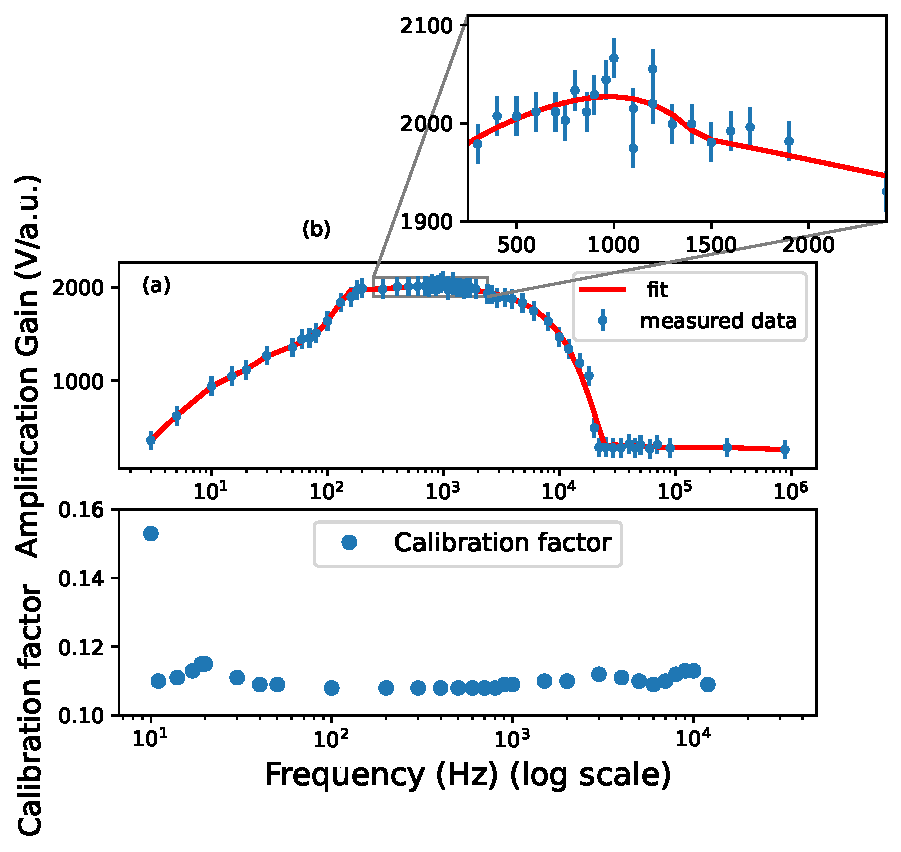
\includegraphics[scale =0.5, trim={5 0 5 0},clip]{JNM-Final Draft/calib.pdf}
\caption{(a) Gain of the voltage amplifier as a function of the frequency of the input signal plotted on a log scale. (b) The gain of the voltage amplifier as a function of the frequency of the input signal on a log scale for frequencies in the range $300$ Hz to $2400$ Hz, where we observe a constant gain of $\sim$2000. The solid red line represents the polynomial fit of order 4 performed on the gain of the voltage amplifier in the given interval. (c) Measured calibration factor of the sound card as a function of the frequency of the generated signal on a log scale. The calibration factor is constant at a value of $\sim0.109 $ for frequencies in the range $100$ Hz to and $7000$ Hz, increases slightly to $0.11 $ for frequencies above $8000$ Hz and increases significantly to a value of $0.155$ for a signal of frequency equal to $10$ Hz. We will choose a bandwidth that does not include low frequencies ($<50Hz$) for which the soundcard does not yield a reliable calibration factor.}
\label{calib} 
\end{figure}

The amplifier includes  multiple internally compensated operational amplifiers, that tend to be designed to have gain that rolls off at some frequency in order to ensure that the circuits in which they are used do not oscillate or go unstable when used in a negative-feedback configuration. Hence, the gain of a voltage amplifier changes with the frequency of the input signal and has a specific frequency range for which it delivers an optimal gain\cite{6908352}. A frequency analysis of the amplifier’s gain was therefore performed and the gain curve we obtained was then fitted to a polynomial function. This allowed us to derive a mathematical expression for $g(f)$ (namely a piecewise function) that describes the gain as a function of frequency and then use it to compute the gain integral $G(f_1, f_2)= \int_{f_1}^{f_2} g^2(t)\,df\ $ over a certain bandwidth. A sinusoidal function generator was used to calibrate the gain curve and a Stereo Audio USB External Sound Card, as well as an oscilloscope, were deployed to read the RMS voltage of the amplified signal. One of the advantages of using the soundcard to measure the amplified noise signal is that we can display the converted sound signal using the software Audacity. As the calibration factor of the soundcard fluctuates with the frequency of the input signal as well, a frequency analysis of the calibration factor was necessary before using the soundcard as a tool to measure the RMS voltage signal. The frequency dependence of the calibration factor was derived and is displayed in [Fig.~\ref{calib}]. The uncertainty in the value of the square of the gain of the amplifier was determined by simple error propagation, yielding $\sigma_{g^2}=\pm5.2$. Analogously, the uncertainty in the calibration factor was derived to be $\pm 0.018V$. 


\begin{figure}
\centering
\begin{subfigure}[a]{0.55\textwidth}
   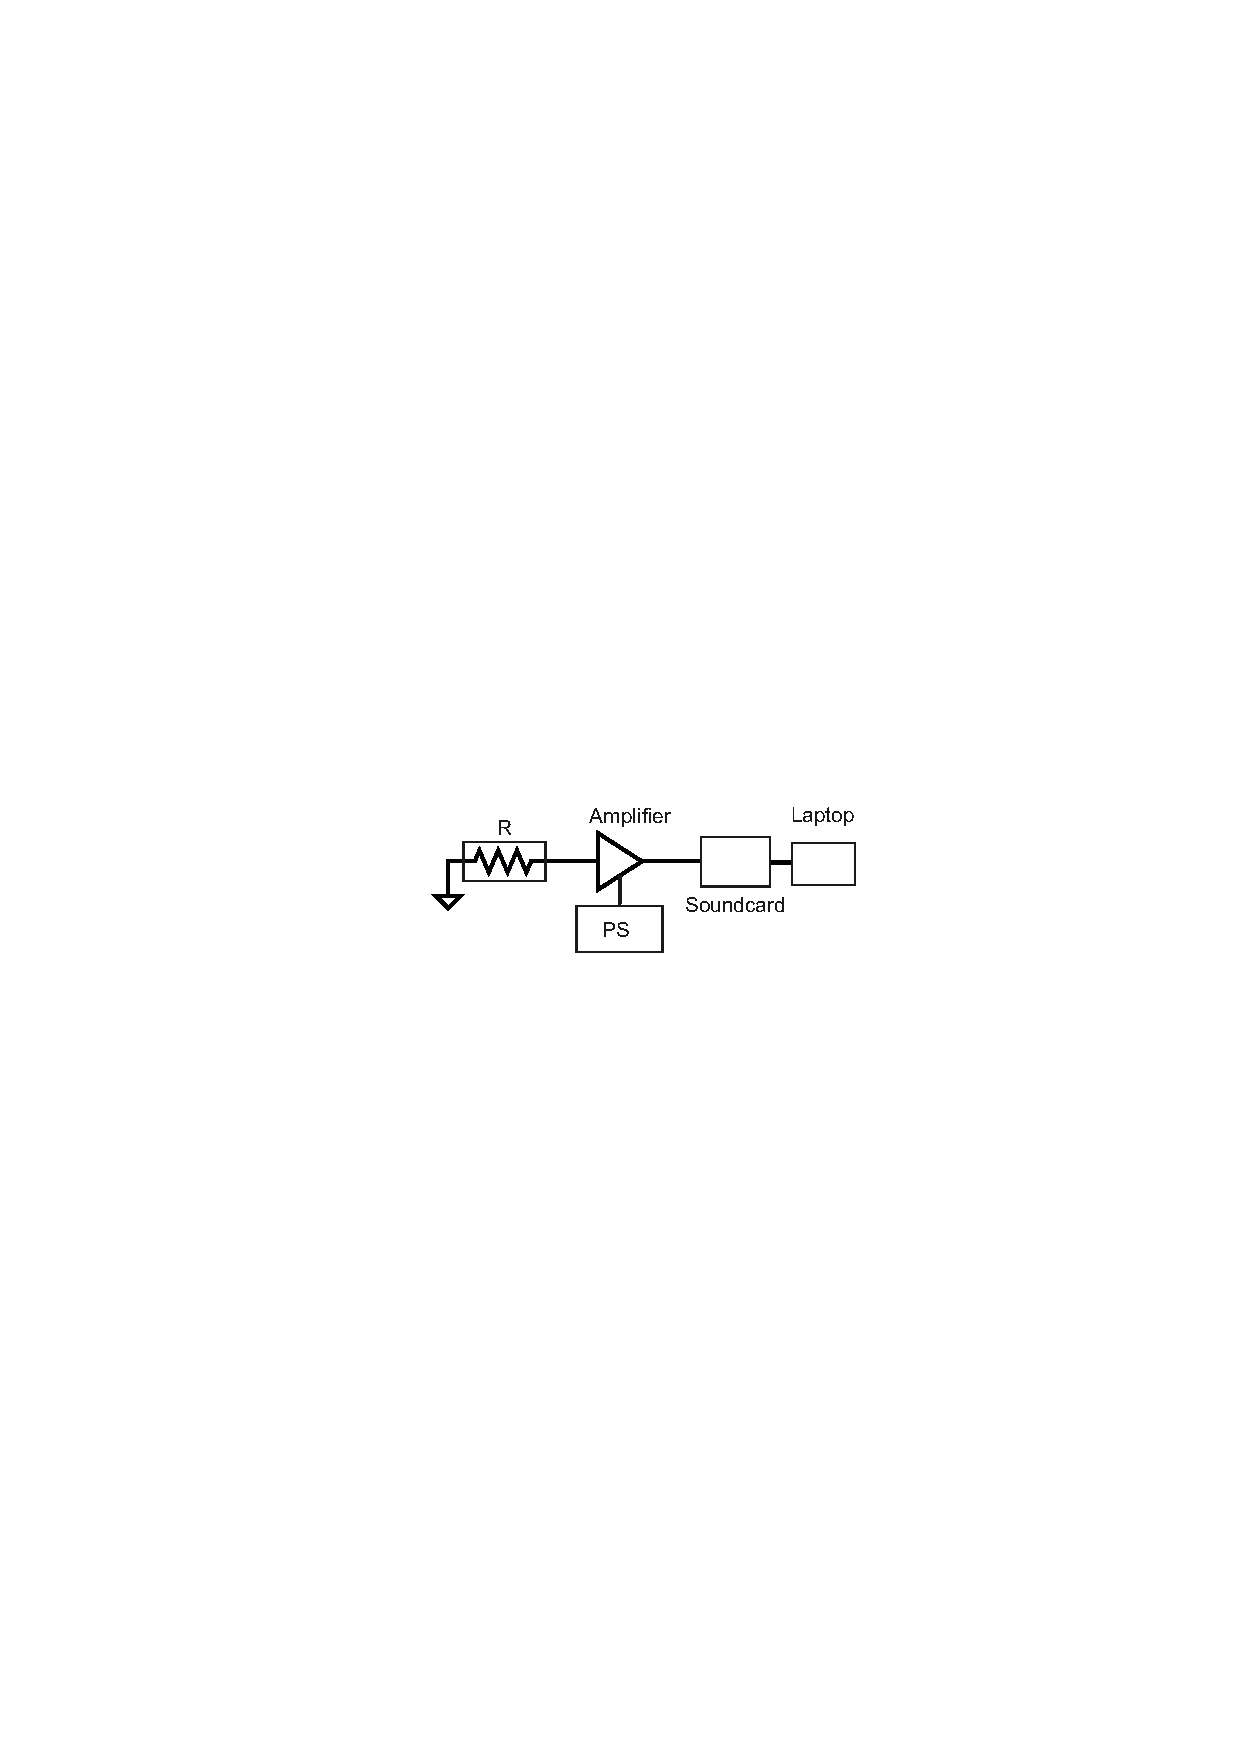
\includegraphics[scale =0.8, trim={200 375 0 375},clip]{JNM-Final Draft/Circuit_diagram.pdf}
   \label{fig:circuit} 
\end{subfigure}

\begin{subfigure}[b]{0.55\textwidth}
   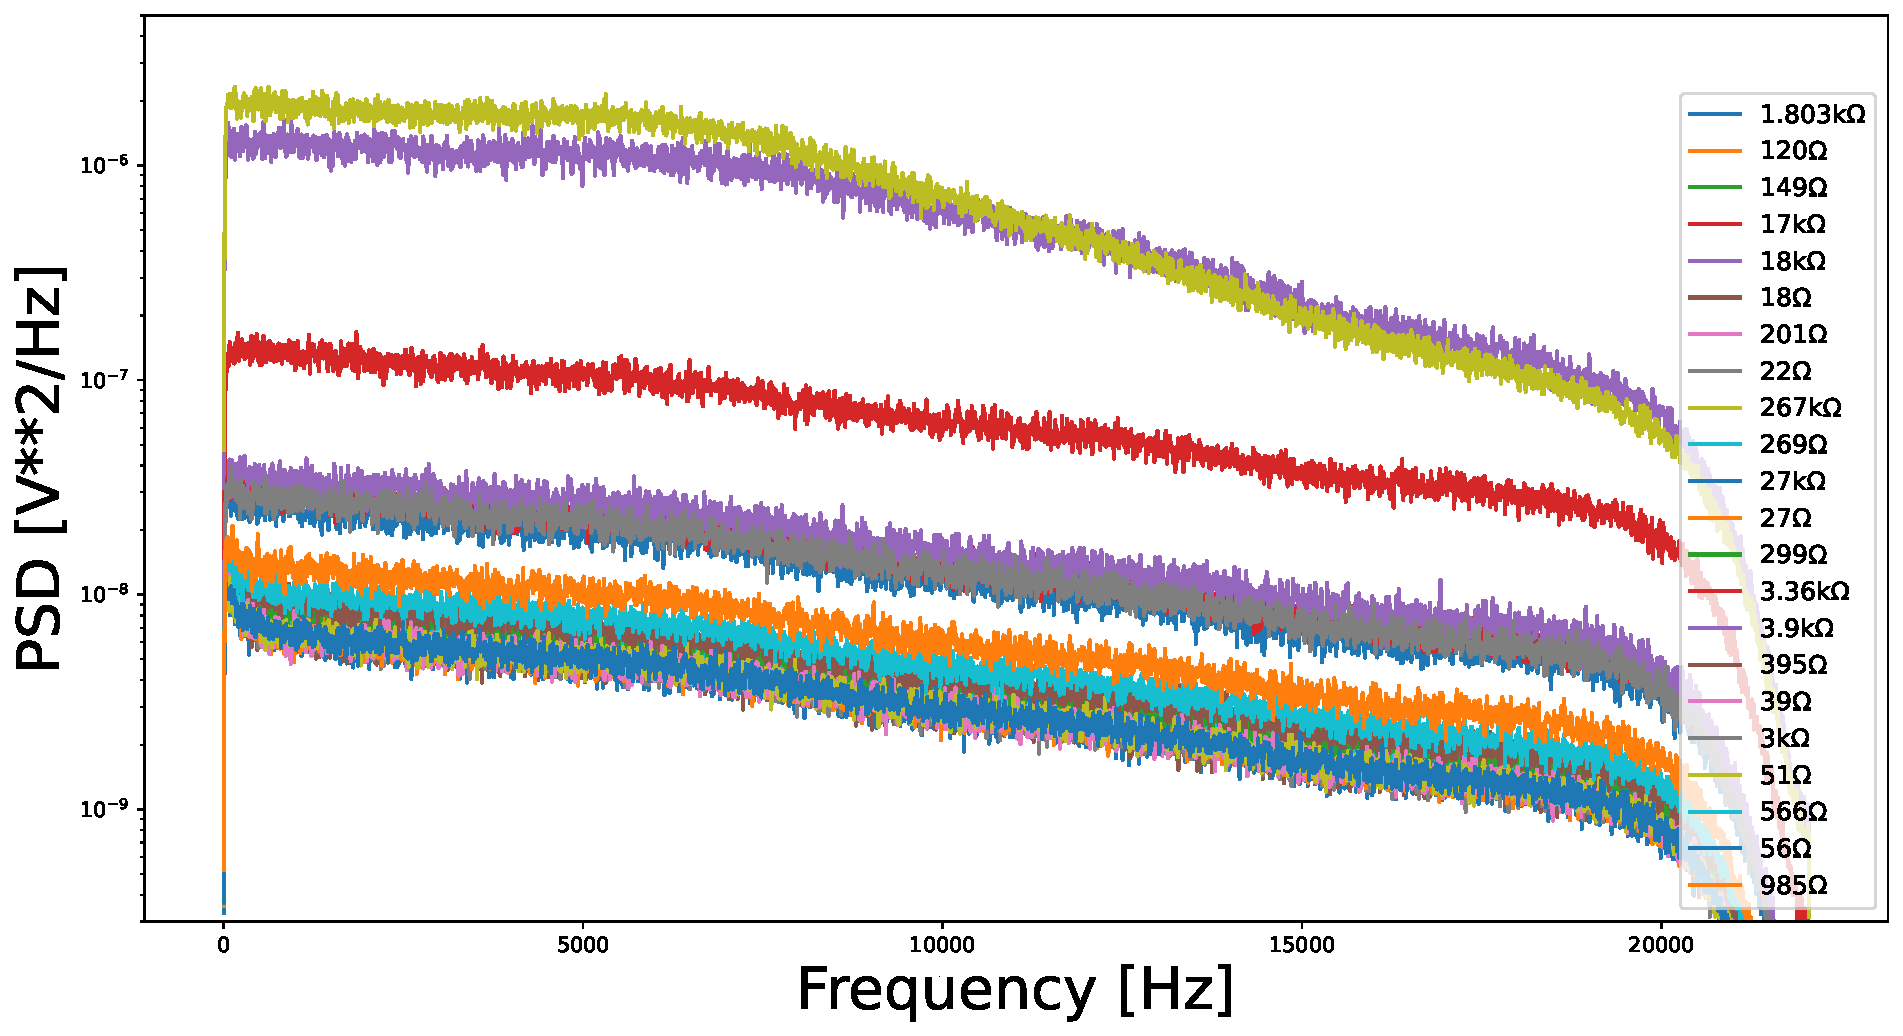
\includegraphics[scale =0.3 ,trim={200 50 -100 0}]{JNM-Final Draft/comparison.pdf}
   \caption{}
   \label{fig:powerspectra}
\end{subfigure}

\caption{(a) Schematic experimental setup. A resistor $R$ inside a copper tube is connected via a BNC cable to a voltage amplifier connected to a power source $PS$ (battery). The output voltage of the amplifier is measured by a sound card connected via a USB cable to a laptop. (b) Semilog plot of the power spectral density of the RMS voltage fluctuations for different resistors ranging from 18 $\Omega$ to 226 $k\Omega$ versus frequency. In the power spectral density plot for resistors with lower resistance, we observe an almost flat power spectral density that is characteristic of Johnson noise (and of any type of "white noise"). As the resistance increases, the power spectral density plot becomes steeper, in agreement with the fact that for small resistances, the contribution of Johnson noise to the total noise across the resistor is significant, while it becomes less significant for larger values of resistance $R$ where current noise starts becoming the dominant source of noise.}
\label{fig:circuit} 
\end{figure}

Once we have performed the frequency analysis of the amplifier and the calibration of the soundcard and assessed the uncertainties of both measurements, we can use the soundcard to measure the amplified RMS voltage fluctuations across various resistors. The recorded voltage fluctuations were exported as $.wav$ files such that we could analyse the signal for a given resistance $R$ by computing the power spectral density of it using a periodogram. The average of the power spectral density for the RMS voltage signal across each resistor (for a given bandwidth) yields the average noise $V_{out}$ per unit frequency measured across each resistor. 
However, by connecting the resistor $R$ to the input of an amplifier, we are confronted with a new circuit configuration that introduces two additional and distinct noises, generated by the amplifier itself: current and voltage noise \cite{article}. If the resistor is connected across the input of a high-gain amplifier with gain function $g(f)$, then the infinitesimal mean-squared voltage measured at the output of the amplifier will now be given by $dV_{out}=g(f)(dV_{JN}+dV_{A}^{in})df$, where $V_{JN}$ represents the random voltage fluctuations due to Johnson noise and $V_{A}^{in}=V_{A}^{IR}+V_{A}^{V}$ the voltage signal resulting from both the current and voltage noise of the amplifier, respectively. Using the fact that uncorrelated noise voltages add in a root-sum-of-squares manner, we can express the total infinitesimal power dissipated by the circuit for an infinitesimal frequency range $df$ by simply adding the infinitesimal contribution of each noise source to the infinitesimal magnitude of the total noise power $dS_{out}$
\begin{equation}
\label{eqn:infinitesimalS}
    dS_{out}=g(f)^2df\times(dS_{JN}+dS_{IR}+dS_{V} (f)). 
\end{equation}
Where $dS_{JN}$ represents Johnson noise, $dS_{IR}$ and $dS_{V}$ current and voltage noise from the amplifier, respectively. 
In Equation \ref{eqn:infinitesimalS}, we have assumed that the voltage noise due to the amplifier is at the input of the amplifier and gets amplified along with the current and Johnson noise. This assumption allows us to derive a simplified model for the total noise measured across each resistor. However, we acknowledge the fact that the mathematical model displayed in Equation \ref{eqn:infinitesimalS} represents an approximation of the real behaviour of the total power dissipated in the circuit. We define the gain integral $G(f_1,f_2)$ to be the integral of the squared fitted gain function $g(f)$ over the bandwidth $(f_1, f_2)$. We calculate the gain integral numerically using Simpson's rule \cite{article} over the same bandwidth we measure the noise over. By integrating Equation \ref{eqn:infinitesimalS} over a certain bandwidth $(f_1, f_2)$, we can express the total noise power of the circuit over a certain frequency range as a function of the gain integral (calculated for the given bandwidth) and add the contribution of each noise to the total magnitude of the noise power $S_{out}=G\times(S_{JN}+S_{IR}+S_{V} (f))$, where $G(f_1, f_2)= \int_{f_1}^{f_2} g^2(t)\,df\ $, $S_{JN}$ represents the power dissipated due to Johnson noise, $S_{IR}$ and $S_{V}$ the current and the voltage noise of the amplifier, respectively, over a bandwidth $(f_1,f_2)$.

 By using Ohm’s law $V=IR$ and Nyquist's theorem (\ref{eqn:2}), we can modify Equation \ref{eqn:infinitesimalS} and model the total noise power such that we can distinguish between the three distinct types of noise involved. Let Johnson noise per bandwidth be $S_{JN}= 4 k_bRT$ and current noise be $S_IR=(V_{A}^IR )^2 =(IR)^2=S_I R^2$, then 
\begin{equation}
\label{eqn:model}
     S_{out} =G\times(4 k_bRT+ S_I R^2+ S_V)  
\end{equation}

We observe that only the first two terms are dependent on the resistance at the input of the circuit. While current noise $S_{IR}$ grows quadratically as a function of $R$, Johnson noise $S_{JN}$  is in a linear relationship with $R$. Thus, by measuring the RMS voltage fluctuations per unit bandwidth across the terminals of different resistors, over a fixed bandwidth, we can derive the power dissipated by each resistor in the circuit and relate it to both the current and Johnson noise with appropriate fitting. As current noise grows quadratically with resistance, we expect it to become the dominant source of noise for large values of $R$. However, we can exploit the fact that there exists a certain range of values for $R$ for which the resistance is small enough in order to observe a significant contribution of Johnson noise to the overall noise $S_{out}$ in the circuit. According to Equation \ref{eqn:equation2}, Johnson noise per bandwidth is equal to $4kbR$ and we can therefore model the contribution of Johnson noise to the total noise as a linear function of resistance $R$. Johnson noise was derived from the noise power (per unit frequency) in the range of R for which there exists a linear relationship between the total noise power of the signal and $R$.

We measured 4 times the RMS voltage fluctuations across 25 different resistors with resistance ranging from $18\Omega$ to $226 k\Omega$. A bandwidth of $1050Hz$ was chosen and kept fixed for all resistors, such that we could use the constant calibration factor $c=0.10$ we previously derived.
We find that $18 \Omega$-$50k\Omega$ represents a range of R where the total noise in the circuit is not dominated yet entirely by the current noise. In fact, a linear relationship between the power noise and the resistance values between $18 \Omega$ and $55.81 k\Omega$ seems to hold. Above $55.81k\Omega$, the contribution by current noise to the total noise $S_{out}$ becomes dominant and we observe that $S_{out}$ starts increasing not linearly anymore. To confirm this and to derive numerical values used to calculate $k_b$, we fit the data for $S_{out}$ to a quadratic polynomial function $f(R)=aR^2+bR+d$, where the first, 2nd and 3rd term represents contributions to the total noise in the circuit by the current, Johnson and voltage noise, respectively. 
\begin{figure}[h]
\centering
\begin{subfigure}{0.5\textwidth}
    \includegraphics[width=\textwidth]{JNM-Final Draft/fitting.pdf}
    \label{fig:first} 
\end{subfigure}

\begin{subfigure}{0.4\textwidth}
    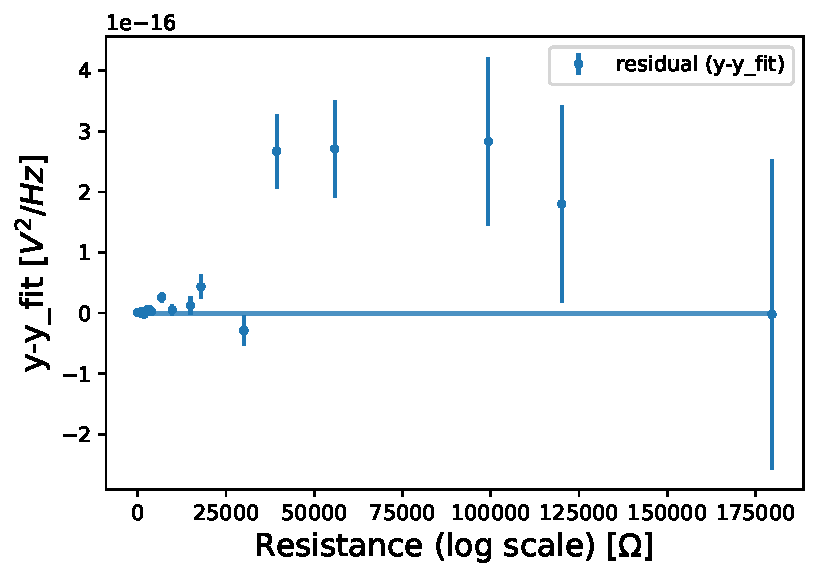
\includegraphics[scale =0.5]{JNM-Final Draft/residuals.pdf}
   \label{fig:second}
\end{subfigure}
\caption{(a) Plot of the measured values for $\frac{V^2_{rms}}{G}$ versus resistance $R$ with the fitted function $f(R)$ for all the resistance values between $18 \Omega$ and $260 \Omega$. (b) Plot of the measured values for $\frac{V^2_{rms}}{G}$ as well as the values of $\frac{V^2_{rms}}{G}$ of the cross-correlated signal versus resistance $R$ with the fitted function $f(R)$ for small values of $R$ where a linear relationship between  $\frac{V^2_{rms}}{G}$ and $R$ holds. The plot shows that the cross-correlated signal differs significantly from the original signal for small values of resistances. (c) A plot of the residuals of the fitted model $f(R)$ versus resistance $R$. The residual plots are randomly distributed around 0 and there is no trend in the residual plot, which suggests that the total noise $\langle dV_{RMS}\rangle ^2$ can be modelled as a quadratic function given by Equation \ref{eqn:model} in this resistance range.}
\label{fig:figures}
\end{figure}
As a final consideration in the numerical derivation of Johnson noise and the Boltzmann constant $k_b$, we need to take into account that we are reading the RMS voltage using a digital soundcard with average calibration factor of $c=0.11 \frac{V}{a.u.}$. The real amplified noise $S_{rms}$ (in units of $\frac{V^2}{Hz}$) is given by $S_{rms}=S_{out}\times c^2$. As we are measuring the noise over the frequency interval $300Hz-1350Hz$ for which we can assume a constant calibration factor $c$, we can simply multiply the values for $S_{out}$ by the value of the calibration factor squared, $c^2=0.0121 \frac{V}{a.u.}$, before fitting it to the function $f(R)$. We will not present the explicit RMS voltages obtained for each resistor, however, we note that the measured RMS voltage, adjusted for gain and the calibration factor, ranged from about $1.74nV$ for the $18\Omega$ resistor to about $51.7 nV$ for the $226 k\Omega$. We note that the (relative) residual between the measured RMS voltage and the Johnson noise value as predicted by Nyquist, $r=\frac{V_{rms} - \sqrt{4k_bRT)}}{V_rms}$ is smaller for smaller resistance values; in agreement with the fact that Johnson noise becomes less significant as a noise source for larger values of $R$. 



In an attempt to extract Johnson Noise from the total noise in the circuit and derive a more accurate value for the Boltzmann constant $k_b$, we will proceed by computing the cross-spectral-density ($CSD$) of the two signals in the right and the left channel of the sound card. As the $CSD$ displays the distribution of power for a pair of signals across a frequency spectrum at any time, it can be used to determine how correlated  two signals are in reference to another \cite{LARIVOIRE20171}. Since both channels of the sound card are perturbed by uncorrelated voltage noise signal, we expect that by computing the cross-correlation of the two different channel signals, we are able to extract the correlated components of the signal, composed of Johnson and current noise, and discard the random-generated voltage noise due to the amplifier. Hence, the real part of the cross-correlated signal will yield the noise contribution solely due to Johnson noise and the current noise (namely $S_{out} =G\times(4 k_bRT+ S_I R^2)$). Moreover, as Johnson noise is the dominant noise for small resistances, we expect that the cross-correlated signal varies significantly from the original one for small resistances, as shown in  \ref{fig:figures}. At higher resistances, where current noise dominates all other forms of noise, the cross-correlated signal will resemble almost the original one, as the process of discarding via $CSD$ voltage noise will not contribute a lot to the change in the total noise recorded by the sound card.

We plot $ \frac{S_{RMS}}{G}$ versus resistance $R$ and fit the measured values for $\frac{S_{RMS}}{G}$ to the fitting function $f(R)=aR^2+bR+d$ using linear regression. After cross-correlation, as the total noise in the cross-correlated does not include voltage noise, we should expect the parameter $d$ to be ideally close to zero, so we will set the initial guess for $d$ to zero. The fit displayed in \ref{fig:figures} suggests an acceptable agreement with the model with a reduced $\chi^2$ value equal to $1.4079$. From the fit, we find that the coefficient $b$ is equal to $(1.641e-20 e^{-20} \pm - 6.977e^{-25})\frac{V^2}{RHz}$. Since $b$ equals the coefficient of the linear term in Equation \ref{eqn:model} and this linear term represents the contribution of Johnson noise $S_{JN}$, we derive that the Johnson noise across each resistor R is given by  $S_{JN}=b\times R$. To illustrate an example, we derive a value for the Johnson noise per unit frequency for the 18$\Omega$ resistor equal to $S_{JN}= 2.597e^{-20}\frac{V^2}{Hz}$, which is close to the value for $S_{JN}$ predicted by Nyquist's theorem ($2.960e^{-20}\frac{V^2}{Hz}$). The coefficient $a$ of the quadratic term is $a=2.378e^{-27} \pm 4.500e^{-30}$ and the constant $d$ is $d=1.694e^{-19} \pm 1.083e^{-20}$. According to Equation \ref{eqn:model}, the quadratic term $S_IR^2$ represents the contribution of current noise so that the fitted coefficient $a$ is equal to $S_I$. For each resistance $R$, the current noise in the circuit will then be given by $S_I\times R^2=a\times R^2$. In the simplified model displayed in Equation \ref{eqn:model}, the constant term $d$ represents $S_v$, namely the contribution of voltage noise, which is independent of resistance, to the total noise. 
Prior to computing the cross-correlation of the signal, we fitted our quadratic model to the original noise signal recorded by the sound card. As the fitted value $d$ for the original signal was obtained to be negative ($-1.845e^{-17}$), we concluded that this value cannot represent the correct average value for voltage noise and that we need to acknowledge the fact that the model in \ref{eqn:model} is not suited to derive a numerical value for the voltage noise. Instead, when fitting the cross-correlated signal to the same quadratic model, we got a fitted value for the parameter $d$ equal to $ 1.694e^{-20} \pm  1.694e^{-21}$. Although not equal to zero as we predicted (as the new signal should ideally not include any contribution from voltage noise), the new fitted value for $d$ is more than 3 magnitudes smaller than the one obtained for the original signal, prior to $CSD$. Hence, we can conclude that $CSD$ proved to be effective in discarding the random-generated voltage noise from the total noise of the signal. Moreover, by introducing cross-correlation, we were able to derive a new fitted function with an associated $\chi^2$ value of $1.487$, which is lower in magnitude compared to the $\chi^2$ value of $2.4079$ associated with the fitted model obtained from the original (non-cross-correlated) power signal. 

Finally, according to Nyquist's model, measurement of the thermal noise $\langle V_{JN}^2 \rangle$ across any resistor provides a means to calculate the Boltzmann constant $k_b$, once we fix the room temperature to be $T=293 K$. Since  $\langle V_{JN}^2\rangle =bR$, where $b$ is the fitted parameter previously derived, we derive a value for the Boltzmann constant equal to $k=\frac{b[\frac{V^2}{RHz}]}{4T[K]} =1.4098e^{-23} \frac{J}{K}$. The absolute error $\simga_{k}$ was calculated using the absolute error in the fitted value for $b$, namely $\sigma_{k} = k\sqrt{\frac{\sigma_{b}}{b}}=6.146e^{-28}\frac{J}{K}$.

In conclusion, our results are in acceptable agreement with both Nyquist's theoretical predictions and the literature value for the Boltzmann constant. Without the cross-correlation analysis, we derive from the measurement of Johnson noise, a value of the Boltzmann constant equal to $ k_b = (1.541e-23e^{-23} \pm 5.938e^{-28})J/K$. A significant improvement in the derived value for $k_b$ was achieved by using the technique of cross-correlation. In fact, by computing the cross-spectral density of the signals inside the two channels of the sound card, we were able to extract the Johnson noise and the current noise from the total noise in the circuit and derive a more accurate value for the Boltzmann constant $k_b$, namely $(1.4098e^{-23} \pm 6.146e^{-28})J/K$. The  $\chi^2$ value of the fitted model also proved to be significantly lower for the cross-correlated signal. 
The value we derived for $k_$ can be improved in future measurements by further reducing the external noise sources as well as by including a larger and broader set of resistance values  across which we can measure Johnson noise. An accurate derivation of voltage noise (which is frequency dependent) was not performed and the fitted parameter $d$ 
can be interpreted as the contribution of voltage noise to the total noise in the circuit.  Nevertheless, we were able to demonstrate the validity of various theoretical aspects concerning Johnson noise (i.e. the fact that it has a flat spectral density and is therefore considered "white noise") as well as deriving a fairly accurate value for the Boltzmann constant $k_b$. 
\end{linenumbers}
\bibliography{main}
\end{document}